%% LaTeX Beamer presentation template (requires beamer package)
%% see http://latex-beamer.sourceforge.net/
%% idea contributed by H. Turgut Uyar
%% template based on a template by Till Tantau
%% this template is still evolving - it might differ in future releases!

\documentclass{beamer}
\usepackage[brazil]{babel}
\usepackage[utf8]{inputenc}
\usepackage{amsfonts}
\usepackage{amsmath}
\usepackage{pgfpages}

% \setbeameroption{show notes}
% \setbeameroption{show notes on second screen=left}

\mode<presentation>
{
    \usetheme{Frankfurt}
    
    \setbeamercovered{transparent}
}


\title{Estudo, Definição e Implementação de Ambiente de Ensino-Aprendizagem com Arquitetura de Agentes e Modelo Multidimensional de Aprendizagem}

% - Use the \inst{?} command only if the authors have different
%   affiliation.
%\author{João Paulo de Freitas Matos}
\author{João Paulo de Freitas Matos\\{\small Orientadora\\ Prof\textordfeminine Dr\textordfeminine Célia Ghedini Ralha}}

%\author{\inst{1}}

% - Use the \inst command only if there are several affiliations.
% - Keep it simple, no one is interested in your street address.
\institute[UnB]
{
    %\inst{1}
    {\Large Universidade de Brasília}\\
    {\small
    Instituto de Ciências Exatas\\
    Departamento de Ciência da Computação}

  %\includegraphics[width=\len@brasiliaw]{#1}\\[.63\len@uacaph]%logo com a largura da palavra Brasilia
      %\@universidade\@lskipoffset{.5}%
          %\@textscale{.5}{\@instituto}\@lskipoffset{.25}%
              %\@textscale{.5}{\@departamento}%


}


\date{12 de março de 2013}


% This is only inserted into the PDF information catalog. Can be left
% out.
%\subject{Talks}



% If you have a file called "university-logo-filename.xxx", where xxx
% is a graphic format that can be processed by latex or pdflatex,
% resp., then you can add a logo as follows:

\pgfdeclareimage[height=0.5cm]{university-logo}{figuras/unb.png}
\logo{\pgfuseimage{university-logo}}



% Delete this, if you do not want the table of contents to pop up at
% the beginning of each subsection:
%\AtBeginSubsection[]
%{
%\begin{frame}<beamer>
%    \frametitle{Sumário}
%    \tableofcontents[currentsection,currentsubsection]
%    \end{frame}
%}

% If you wish to uncover everything in a step-wise fashion, uncomment
% the following command:

%\beamerdefaultoverlayspecification{<+->}

\begin{document}

% ------------- TITLE PAGE -------------
\begin{frame}
\titlepage
\end{frame}
% ------------- TITLE PAGE -------------


% ------------- SUMARIO -------------
\begin{frame}
	\frametitle{Sumário}
	\tableofcontents
\end{frame}


% ------------- Introdução -------------
\section{Introdução}
\begin{frame}
    \frametitle{Introdução}
       \begin{itemize}
	\item Aprendizagem individual;
	\item Modelo multidimensional como representação do aluno;
	\item Determinação do estilo de aprendizagem.
	\item Auxílio na didática do docente;
	\note{.\\-- Tendencia de preferir certa forma de aprender}
	\note{.\\-- Estilo de Aprendizagem}
	\note{.\\-- Afetivo, Cognitivo e Metacognitivo}
    \end{itemize}
\end{frame}


% ------------- Problema -------------
\subsection{Problema}
\begin{frame}
    \frametitle{Problema}
    \begin{itemize}
	\item Arquitetura não apropriada para a inferência do modelo multidimensional;
	\item Abordagem cliente-servidor é desvantajosa.
	\begin{itemize}
		\item Alta complexidade;
		\item Não há representação individualizada em tempo real.
	\end{itemize}
    \end{itemize}
\end{frame}

% ------------- Objetivos -------------
\subsection{Objetivos}
\begin{frame}
    \frametitle{Objetivos}
    \begin{itemize}
	\item \textbf{Objetivo Geral}
        \begin{itemize}
		\item Definir uma arquitetura distribuída com abordagem de Sistema multiagente (SMA), visando a inferência do modelo do aluno.
	\end{itemize}

	\note{.\\-- Auxiliar o processo de ensino-aprendizagem; Criação de insumos - docente - melhor estratégia didática de ensino.}

	\item \textbf{Objetivos Específicos}
	\begin{itemize}
        	\item Projeto da arquitetura geral do SMA, com metodologia apropriada;
		\item Definir e implementar a arquitetura da solução: agentes assistentes de cognição, metacognição e afetivo;
		\item Interface do agente cognitivo com o aluno e o docente; % Propor
	\end{itemize}
    \end{itemize}
\end{frame}

% ------------- Metodologia -------------
\subsection{Metodologia}
\begin{frame}
    \frametitle{Metodologia}
    \begin{itemize}
	    \item Levantamentos bibliográficos:
		\begin{itemize}
			\item Informática na Educação (IE);
			\item Sistemas Multiagente (SMA);
			\item SMA em contextos pedagógicos.
		\end{itemize}
	    \item Levantamentos de metodologias apropriadas para modelagem de SMA.
	    \item Estudo de~\emph{frameworks} para o desenvolvimento.
	    \item Escolha da plataforma~\emph{web} necessária para a interação com o aluno/docente.
    \end{itemize}
\end{frame}

% ------------- Fundamentos -------------
\section{Fundamentos}
\begin{frame}
    \frametitle{Informática na Educação}
     \begin{itemize}
  		\item Inserção do computador no processo de aprendizagem.
  		\item Computador apresenta recursos importantes que auxiliam o ensino-aprendizagem.
		\item Ambientes Virtuais de Aprendizagem
		\note{.\\-- Facilidade de recursos.}
		\note{.\\-- Aluno + objeto de conhecimento: Desenvolvimento cognitivo.}
		\note{.\\-- AVA - Educação a distância. Gerenciamento de cursos, acompanhar progresso do aluno. Falar sobre .}
	\end{itemize}
\end{frame}

\begin{frame}
    \frametitle{Informática na Educação}
     \begin{itemize}
  		\item Modelo Multidimensional: % Compreende as dimensões:
		\begin{itemize}
  			\item Cognitivo;
	  		\item Afetivo;
	  		\item Metacognitivo.
		\end{itemize}
		\note{.\\-- Cognitivo: Faculdade de conhecer, atenção, percepção, pensamento.}
		\note{.\\-- Metacognitivo: Faculdade de conhecer o próprio ato de conhecer, ou, por outras palavras, consciencializar, analisar e avaliar como se conhece.}
		\note{.\\-- Afetivo: Detecção de emoções na interação humano computador.}
  		\item Estilos de Aprendizagem:
		\note{.\\-- Melhor forma de receber e processar as informações.}
		\begin{itemize}
	  		\item Classificam o aluno em uma hierarquia;
  			\item Diversos modelos de estilo;
	  		\item Questionário de Estilo de Aprendizagem. %Inferência Explícita: 
		\end{itemize}
		\item Orientação do docente.
		\note{.\\-- Podem orientar sobre a melhor forma dos seus alunos aprender.}
	\end{itemize}
\end{frame}

\begin{frame}
    \frametitle{Agentes e Sistema Multiagente}

	\begin{itemize}
  		\item Agentes~\cite{novig95};
  		\item Ambiente;
  		\item Sensor;
		\item Características:
		\begin{itemize}
  			\item Proatividade;		
	  		\item Reatividade;		 
	  		\item Habilidade Social.	 
		\end{itemize}
		\note{.\\-- Não necessita de interências externas para agir.}
		\note{.\\-- Reage à um estímulo do ambiente.}
		\note{.\\-- Pode interagir e influenciar outros agentes.}
	\end{itemize}

    \begin{figure}[h]
    	\centering 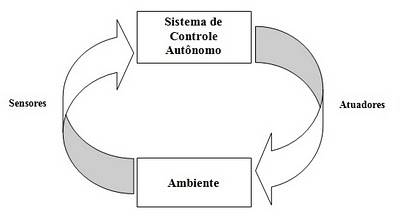
\includegraphics[scale=0.45]{figuras/agente.jpg}
    	\caption{Funcionamento de agentes~\cite{wooldridge04}}
	\label{agente} 
    \end{figure}
\end{frame}

\begin{frame}
    \frametitle{Sistema Multiagente}

	\begin{itemize}
  		\item Interação - Vários agentes em um ambiente;
		\begin{itemize}
	  		\item Objetivos Distintos;
  			\item Capacidade de decomposição dos problemas;
	  		\item Autonomia de decisões. % Agentes podem ou não cooperar com outros agentes.
		\end{itemize}
  		\item Comunicação - Protocolos:
		\begin{itemize}
	  		\item KQML
  			\item FIPA~\emph{Agent Comunication Language} (ACL).
		\end{itemize}
	  	\item Ontologias.
		\note{.\\-- Representar a natureza do ser, existência ou realidade.}
	\end{itemize}

\end{frame}


\begin{frame}
    \frametitle{Metodologias de Modelagem de SMA}

	    \begin{itemize}
  		\item Diferem de projetos orientados à objetos.
  		\item Alternativa: \emph{Multiagent Multiagent Systems Engineering} (MASE).
		\begin{itemize}
	  		\item Série de modelos gráficos.
	  		\item Requisitos e metas iniciais.
  			\item Iterativa.
		\end{itemize}
	    \end{itemize}

\end{frame}

\begin{frame}
    \frametitle{Metodologias de Modelagem de SMA}

	    \begin{itemize}
  		\item Duas fases.
  		\item Análise:
		\begin{itemize}
	  		\item Capturar metas;
	  		\item Desenvolvimento dos casos de uso;
			\item Refinar Regras.
		\end{itemize}
		\item \emph{Design}:
		\begin{itemize}
	  		\item Classes;
	  		\item Conversações;
			\item Montar agentes;
			\item Design do Sistema.
		\end{itemize}
	    \end{itemize}

\end{frame}

\begin{frame}
    \frametitle{Ferramentas - JADE}

	\begin{itemize}
  		\item Desenvolvimento do SMA: JADE.
		\item Simplificação.
		\item Arquitetura distribuída.
	     \begin{figure}[h]
	    	\centering 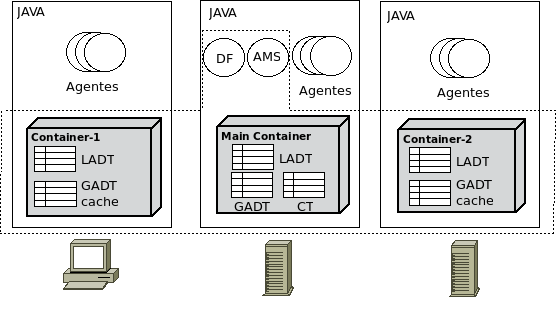
\includegraphics[scale=0.5]{../images/arquitetura-jade.png}
    		\caption{Arquitetura do~\emph{framework} JADE}
		\label{arquiteturaJade} 
	    \end{figure}
	\end{itemize}
\end{frame}

\begin{frame}
    \frametitle{Ferramentas - Seam}

	\begin{itemize}
  		\item Desenvolvimento da interface web: Jboss Seam.
		\item Integra as principais ferramentas consolidadas~\ref{pilhaSeam}.
		\item Geração automática de código.
	     \begin{figure}[h]
	    	\centering 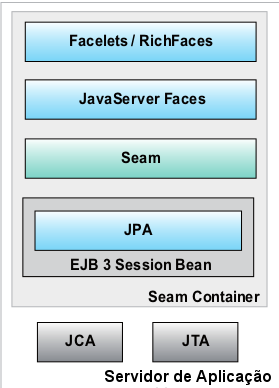
\includegraphics[scale=0.37]{../images/servidor-app-seam.png}
    		\caption{Pilha de Aplicações do Seam}
		\label{pilhaSeam} 
	    \end{figure}
	\end{itemize}
\end{frame}

% ------------- Proposta -------------
\section{Proposta}
\subsection{Modelagem}

\begin{frame}
    \frametitle{Modelagem - MASE}
    \begin{itemize}
        \item Atores;
        \item Interação com os atores;
        \item Requisitos;
	\item Nome da solução: Frank;
	\note{.\\-- Quem são atores?}
	\note{.\\-- Como interagem?}
    \end{itemize}
\end{frame}

\begin{frame}
    \frametitle{Modelagem - MASE}
    \begin{itemize}
        \item Regras:
	\begin{itemize}
		\item StudentInterface;
		\item WebServiceInterface;
		\item Manager;
		\item StudenWorkgroup;
		\item CognitiveAction;
		\item MetacognitiveAction;
		\item AffectiveAction;
		\item LearningMethodAnalyzer.
	\end{itemize}
    \end{itemize}
\end{frame}

\begin{frame}
    \frametitle{Modelagem - MASE}
    \begin{itemize}
        \item Regras e Tarefas:
	 \begin{figure}[h]
    		\centering 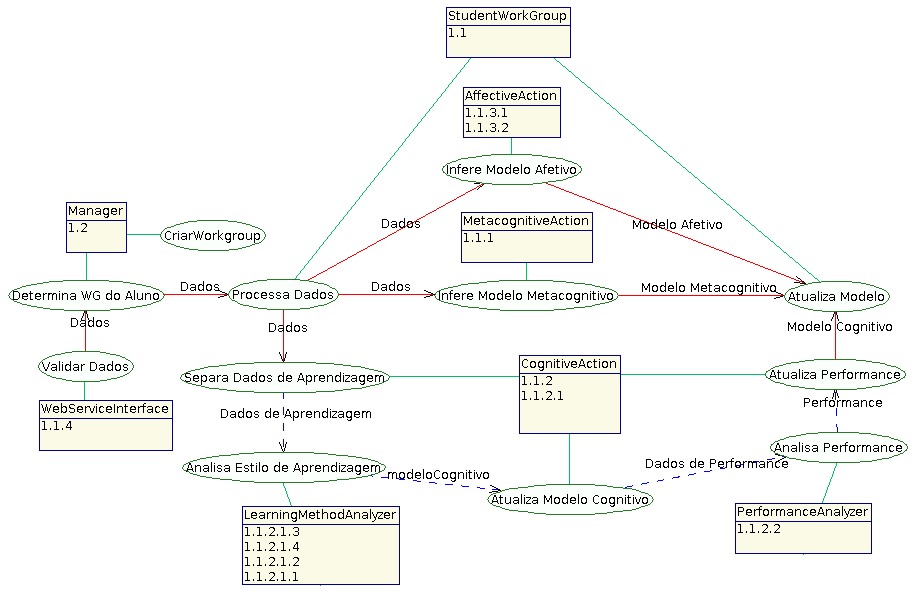
\includegraphics[scale=0.3]{../images/mase-role-model.png}
    		\caption{Mase Role Model}
		\label{maseRoleModel} 
	\end{figure}
    \end{itemize}
\end{frame}

\begin{frame}
    \frametitle{Modelagem - MASE}
    \begin{itemize}
        \item Agentes e conversações:
	 \begin{figure}[h]
    		\centering 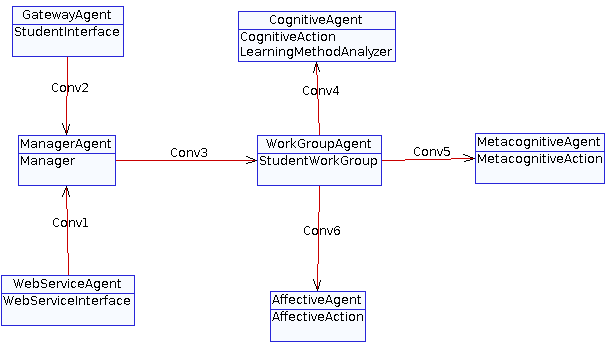
\includegraphics[scale=0.3]{../images/agent-class-diagram.png}
    		\caption{Diagrama de Classes de Agentes}
		\label{agentClassDiagram} 
	\end{figure}
    \end{itemize}
\end{frame}

\subsection{Arquitetura}
\begin{frame}
    \frametitle{Arquitetura - Aspectos}
    \begin{itemize}
        \item Duas aplicações: Frank Web e SMA.
        \item Aspectos:
	\begin{itemize}
		\item Maior Distribuição;
		\item Menor Complexidade;
		\item Menor Dificuldade;
	\end{itemize}
    \end{itemize}
\end{frame}

\begin{frame}
    \frametitle{Arquitetura}
    \begin{figure}[h]
    	\centering 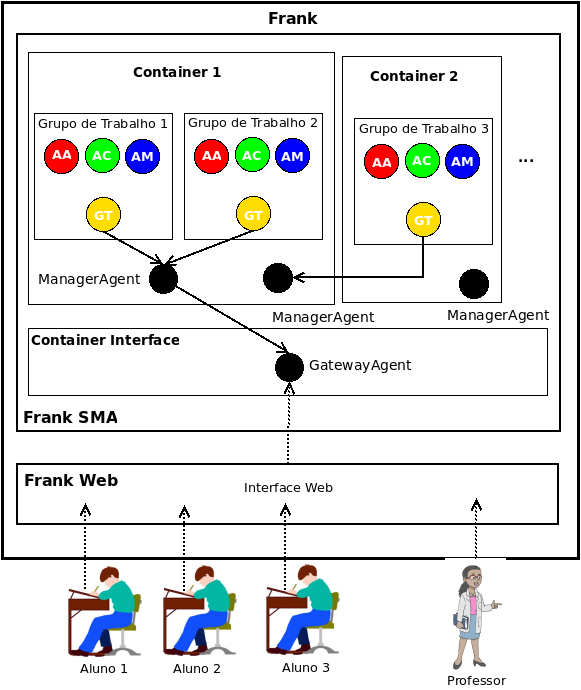
\includegraphics[scale=0.3]{../images/arquitetura-frank.png}
	\caption{Arquitetura Frank}
	\label{arquiteturaFrank} 
    \end{figure}
\end{frame}

\begin{frame}
    \frametitle{Arquitetura}
    \begin{itemize}
        \item Frank Web: Divisão em camadas - MVC.
	\item Servidor de Aplicações.
        \item Autenticação conjunta com SMA.
    \end{itemize}
\end{frame}

\begin{frame}
    \frametitle{Arquitetura - Integração}
    \begin{itemize}
        \item \emph{Container} específico;
	\item \emph{DynamicJadeGateway} no início da plataforma;
	\item Plataforma~\emph{web} é independente das mensagens;
    \end{itemize}
\end{frame}

\begin{frame}
    \frametitle{Arquitetura - Integração}
    \begin{itemize}
	\item Conexão por objetos serializados;
	\item Implementação de Comandos:
	\begin{itemize}
        	\item AnswerCommand
        	\item CreateAgentCommand
        	\item DestroyAgentCommand
        	\item DimensionCommand
        	\item ProcessQuestionnaireCommand
        	\item RequestCognitiveModelCommand
	\end{itemize}
    \end{itemize}
\end{frame}

\subsection{Experimentações}
\begin{frame}
    \frametitle{Experimentações}
    \begin{itemize}
        \item No trabalho, dois cenários:
	\begin{itemize}
		\item Aluno: Inferência do estilo de aprendizagem.
		\item Docente: Verificação de estilos de aprendizagem.
	\end{itemize}
    \end{itemize}
\end{frame}

\begin{frame}
    \frametitle{Experimentações - Fluxo do Aluno}
    \begin{figure}[h]
    	\centering 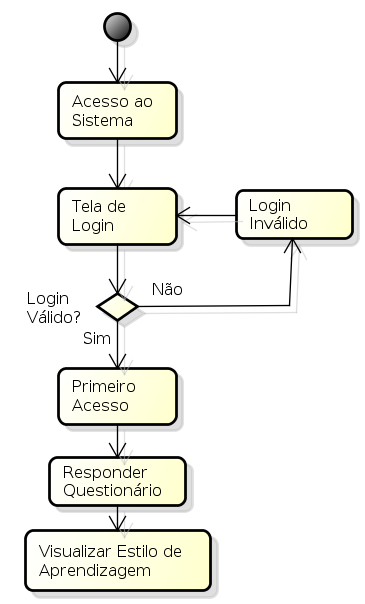
\includegraphics[scale=0.3]{../images/fluxo-aluno.png}
	\caption{Fluxo do Aluno}
	\label{arquiteturaFrank} 
    \end{figure}
\end{frame}

\begin{frame}
    \frametitle{Experimentações - Fluxo do Docente}
    \begin{figure}[h]
    	\centering 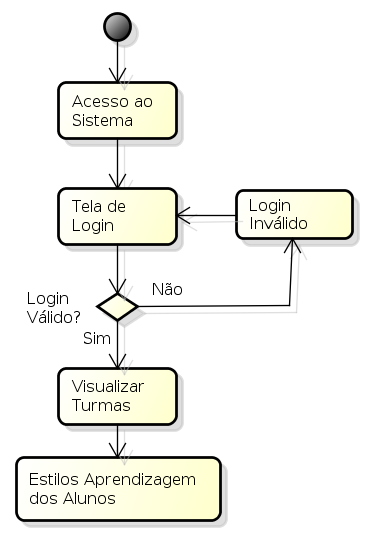
\includegraphics[scale=0.3]{../images/fluxo-docente.png}
	\caption{Fluxo do Aluno}
	\label{arquiteturaFrank} 
    \end{figure}
\end{frame}

\begin{frame}
    \frametitle{Experimentações - Demonstração}
    \begin{itemize}
        \item Demonstração.
    \end{itemize}
\end{frame}

% ------------- Trabalhos Correlatos -------------
\section{Trabalhos Correlatos}
\begin{frame}
    \frametitle{Trabalhos Correlatos}
    \begin{itemize}
        \item Agente Inteligente no Apoio ao Ensino-Aprendizagem~\cite{soaresagente}:
	\begin{itemize}
	        \item Interação com humanos.
	        \item Não é voltada para a abordagem multidimensional;
	        \item Não prevê a inferência de dados vindos de outros AVA.
	\end{itemize}
	\item FIPA - Ferramenta de Identificação de Aprendizes~\cite{bativa2011}:
	\begin{itemize}
	        \item Identificação de estilos de aprendizagem.
	        \item Arquitetura distinta - Cliente-servidor.
	\end{itemize}

    \end{itemize}
\end{frame}

\begin{frame}
    \frametitle{Trabalhos Correlatos}
    \begin{itemize}
        \item SEMEAI~\cite{geyer2001semeai}:
	\begin{itemize}
	        \item Ensino adaptado;
	        \item Não foca no modelo multidimensional;
	\end{itemize}
	\item EDULIVRE~\cite{rabelo2010identificacao}:
	\begin{itemize}
	        \item Não é multiagente.
	        \item Desenvolvido como AVA.
	\end{itemize}

    \end{itemize}
\end{frame}

% ------------- Conclusòes e Trabalhos Futuros -------------
\section{Conclusões e Trabalhos Futuros}
\begin{frame}
    \frametitle{Conclusões}
    \begin{itemize}
        \item Contribuição para a área de IE:
	\note{.\\-- Através de uma plataforma de ensino-aprendizagem que visa auxiliar a didática de ensino do docente ao perceber a melhor forma que seus estudantes podem aprender.}
	\begin{itemize}
	        \item Auxílio a docentes;
	        \item Auxílio a alunos.
	\end{itemize}
    \end{itemize}
\end{frame}

\begin{frame}
    \frametitle{Trabalhos Futuros}
    \begin{itemize}
        \item Modelar ontologias: Modelo metacognitivo e afetivo;
        \item Aprofundar características dos agentes; % habilidade social, interação entre workgroups
        \item Integração com diversos AVA;
	\item Validação da arquitetura em ambiente real;
        \item Plataforma Web: Maior controle sobre SMA.
    \end{itemize}
\end{frame}


% ------------- REFERENCIAS -------------

\nocite{fabriciobuzzeto,weiser2,saocarlos,yang,hewitt,violajones}

\section{Referências}

\frame[allowframebreaks]{
  \frametitle{Referências}
  \bibliographystyle{plain}
  \bibliography{bibliografia}
}

\begin{frame}
    \frametitle{ }
    \centerline{Obrigado!}
    \centerline{Dúvidas.}
\end{frame}

\end{document}
